\chapter{Introdução à construção de compiladores}

\section{Introdução}

Neste capítulo apresentamos uma visão geral da construção
de compiladores, focando em suas diferentes etapas e nos
diferentes resultados produzidos por cada uma delas.

\section{O desafio da compilação}

Um compilador é um programa que traduz uma linguagem,
denominada origem, para outra, a linguagem de destino.
A tradução não é uma tarefa fácil quando as linguagens
de origem e de destino são muito diferentes. Em um compilador
clássico, a linguagem de origem é uma linguagem de
programação projetada para ser compreensível por humanos,
enquanto a linguagem de destino é uma linguagem assembly
ou linguagem de máquina projetada para ser executada de
forma eficiente pelo hardware. No entanto, outras traduções
são úteis e utilizadas na prática. Por exemplo, o compilador
Java compila o código-fonte Java para código da Máquina
Virtual Java (JVM) (chamado \emph{bytecode}), e o sistema
de tempo de execução da JVM possui um segundo compilador,
\emph{just-in-time} (JIT), que traduz o bytecode executado
com frequência em código de máquina que o processador pode
executar diretamente.

Precisamos de um compilador para executar programas? Não,
os programas podem ser executados usando um interpretador.
Por exemplo, o bytecode Java é executado por um interpretador
JVM que simula a execução de uma máquina hipotética. No
entanto, os interpretadores de software são muito menos
eficientes do que o hardware de um processador, portanto, o
código compilado tende a ser executado pelo menos dez vezes
mais rápido do que o código interpretado. (Na verdade, um
  processador é simplesmente uma implementação de hardware
de um interpretador.) Essa vantagem de desempenho também
significa que o código compilado consome dez vezes menos
energia e gera dez vezes menos calor. Claro, a etapa de
compilação do código em si pode exigir muito poder
computacional, então, se você for executar um programa
apenas uma vez, é melhor interpretá-lo. A compilação faz
sentido para programas que serão executados muitas vezes.

O código-fonte e o código-alvo são geralmente bastante diferentes. O
código-fonte é otimizado para que humanos o leiam e modifiquem. Ele
tenta, até certo ponto, corresponder às noções humanas de linguagem e
possui redundância para ajudar a prevenir erros de programação. O
código-fonte suporta análise e raciocínio, seja por humanos ou por
algoritmos. O código-alvo, por outro lado, geralmente é otimizado
para interpretação eficiente. Ele é compacto, pouco legível e não
desperdiça espaço com redundância. O código-alvo frequentemente
descarta grande parte da estrutura de alto nível do código-fonte,
tornando-o difícil de interpretar.

Mais importante para os compiladores do que o desempenho do código
gerado é a sua correção. Depurar código já é bastante difícil quando
se pode confiar no compilador; se os erros podem ter sido inseridos
pelo próprio compilador, a depuração torna-se verdadeiramente árdua.
As diferenças entre as linguagens de origem e de destino também
dificultam demonstrar que o compilador está a executar a sua função
corretamente. Curiosamente, é possível definir com precisão
matemática o que significa um compilador estar correto, desde que
exista uma semântica definida tanto para a linguagem de origem como
para a de destino: uma descrição matemática do comportamento de ambas
as linguagens. De facto, vários compiladores foram desenvolvidos
juntamente com provas de correção, inclusive provas que podem ser
verificadas automaticamente para garantir que foram construídas
corretamente. Desenvolver compiladores com este elevado grau de
garantia não é o nosso objetivo aqui, mas a abordagem que adotamos,
de especificar precisamente diferentes partes do processo de
compilação, é útil para atingir esse objetivo.

\section{Exemplo de passos feitos por um compilador}

Para ter uma ideia do trabalho que um compilador realiza, considere a
seguinte função curta implementada na linguagem de origem que
usaremos neste curso. Sua sintaxe é semelhante à de várias linguagens
populares, portanto, deve ser fácil de entender.

\begin{minted}{js}
findIndex(a:int[]): int {
    n:int = length a
    i:int = 0
    while i < n {
        if a[i] == i+1 {
            return i
        }
        i = i + 1
    }
    return -1
}
\end{minted}

Um compilador não otimizador poderia traduzir o código acima para
código assembly x86-64, como mostrado abaixo. As variáveis
do programa são armazenadas na pilha de
execução e acessadas por meio de operandos de memória. Por exemplo, a
variável \haskell|a| é armazenada no endereço de
memória \asm|rbp - 16|, onde
\haskell|rbp| é um registrador que aponta para o topo
do frame de pilha atual. Também é importante notar que a estrutura de
controle do código-fonte de alto nível, como a instrução
\javascript|while|, foi substituída por instruções de
desvio de baixo nível, como \asm|jne| e
\asm|jmp|.

\begin{verbatim}
findIndex:
    push    rbp
    mov rbp, rsp
    mov [rbp - 16], rdi
    mov rax, [rbp - 16]
    mov rax, [rax - 8]
    mov [rbp - 24], rax
    mov qword ptr [rbp - 32], 0
L1:     mov rax, [rbp - 32]
    cmp rax, [rbp - 24]
    jge L6
    mov rax, [rbp - 16]
    mov rcx, [rbp - 32]
    mov rax, [rax + 8*rcx]
    mov rcx, [rbp - 32]
    add rcx, 1
    cmp rax, rcx
    jne L4
    mov rax, [rbp - 32]
    mov [rbp - 8], rax
    jmp L7
L4:     jmp L5
L5:     mov rax, [rbp - 32]
    add rax, 1
    mov [rbp - 32], rax
    jmp L1
L6:     mov qword ptr [rbp - 8], -1
L7:     mov rax, [rbp - 8]
    pop rbp
    ret
\end{verbatim}

O código não otimizado é mais ineficiente do que o código que um
programador de assembly experiente poderia produzir, mas um bom
compilador otimizador geralmente consegue igualar ou melhorar o
código escrito manualmente, gerando um código como o mostrado a seguir.
As variáveis são armazenadas inteiramente em registradores, o compilador
fez um trabalho melhor ao
escolher instruções eficientes e as instruções associadas ao
gerenciamento da pilha foram removidas, pois a pilha não é utilizada.

\begin{verbatim}
findIndex:
    mov rcx, [rdi - 8]
    xor edx, edx
L1:     cmp rcx, rdx
    je  L2
    lea rax, [rdx + 1]
    cmp rax, [rdi + 8*rdx]
    mov rdx, rax
    jne L1
    dec     rax
    ret
L2:     mov rax, -1
    ret
\end{verbatim}

O compilador geralmente não termina a tarefa de gerar o código de
máquina; essa etapa é deixada para o montador (assembler). O
resultado da montagem do código assembly otimizado acima é a seguinte
sequência de bytes de código de máquina, expressa em hexadecimal, com
suas posições mostradas em hexadecimal na coluna da esquerda e o
código assembly correspondente mostrado à direita. Observe que os
rótulos no código assembly foram substituídos por deslocamentos hexadecimais.

\begin{verbatim}
0: 48 8b 4f f8                      mov rcx, [rdi - 8]
4: 31 d2                            xor edx, edx
6: 48 39 d1                         cmp rcx, rdx
9: 74 11                            je  0x1c
b: 48 8d 42 01                      lea rax, [rdx + 1]
f: 48 3b 04 d7                      cmp rax, [rdi + 8*rdx]
13: 48 89 c2                        mov rdx, rax
16: 75 ee                           jne 0x6
18: 48 ff c8                        dec rax
1b: c3                              ret
1c: 48 c7 c0 ff ff ff ff            mov rax, -1
23: c3                              ret
\end{verbatim}

\section{Estrutura de um compilador}

Pode parecer quase mágico que seja possível traduzir código-fonte
para código de baixo nível eficiente e correto, e ainda mais
surpreendente que isso possa ser feito com relativa rapidez. A
principal ideia que torna a tradução de alta qualidade viável é não
fazê-la de uma só vez. A maneira de resolver um problema complexo
geralmente é dividi-lo em problemas menores e mais fáceis, e com os
compiladores não é diferente.

Em vez de traduzir diretamente do código-fonte (um fluxo de bytes)
para o código-alvo (outro fluxo de bytes), definimos uma sequência de
fases de compilação, cada uma representando o programa original de
uma maneira diferente. Essencialmente, entre as linguagens de origem
e destino, definimos uma sequência de linguagens intermediárias que
se situam entre a origem e o destino, e são projetadas para a
conveniência da fase de compilação atual.

Para entender melhor como isso funciona, vejamos como um trecho simples
de um programa é representado em cada fase do compilador:

\begin{minted}{java}
if (val >= 0) pos = val
\end{minted}

\section{Análise léxica}

O primeiro passo na compilação é transformar o programa de entrada,
representado como uma sequência de bytes ou caracteres, em uma
estrutura de dados em árvore que suporte as fases posteriores do
compilador. A análise léxica divide a entrada em uma sequência de
tokens (ou lexemas). Essas são as ``palavras'' do programa. Espaços
em branco e outros separadores de tokens são descartados.

A imagem abaixo ilustra o resultado da análise léxica para o trecho
de programa apresentado anteriormente.

\begin{figure}[H]
  
\includegraphics[scale=0.4]{./chapters/lexical.png}
  \centering
\end{figure}

\section{Análise sintática}

O próximo passo é a análise sintática, que cria uma estrutura em
árvore que captura a sintaxe do programa, descartando elementos
sintáticos como parênteses que não afetam o significado do programa.
O resultado desta fase é uma árvore sintática abstrata. Na figura
seguinte, apresentamos a árvore de sintaxe para nosso programa de exemplo.

\begin{figure}[H]
  
\includegraphics[scale=0.4]{./chapters/syntax-tree.png}
  \centering
\end{figure}

\section{Análise semântica}

A análise semântica completa a tarefa de determinar se o código-fonte
representa um programa válido. Frequentemente, envolve a verificação
de tipos. Informações adicionais sobre o programa podem ser coletadas
durante essa fase, como os tipos de expressões do programa. Essas
informações podem ser usadas para enriquecer a árvore sintática
abstrata. Na figura seguinte, apresentamos a árvore de sintaxe
contendo informação de tipos sobre todos os elementos do código.

\begin{figure}[H]
  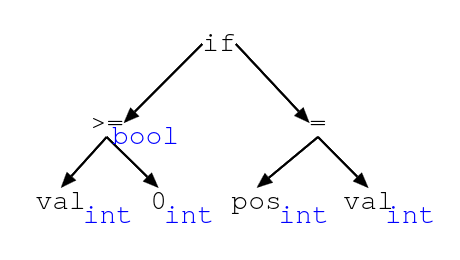
\includegraphics[scale=0.5]{./chapters/annotated-tree.png}
  \centering
\end{figure}

\section{Geração de código}

Após as etapas de análise, o compilador gera novas representações do
programa. Normalmente, há uma fase inicial de geração de código que
produz uma representação intermediária (RI) do programa. Uma fase
posterior do compilador gera o código alvo. Quando a linguagem alvo é
código assembly, essa fase é chamada de seleção de instruções.

Uma representação intermediária comum é um \emph{grafo de fluxo de
controle}. A representação como grafo de fluxo de controle do trecho
de código exemplo é apresentada na figura abaixo.

\begin{figure}[H]
  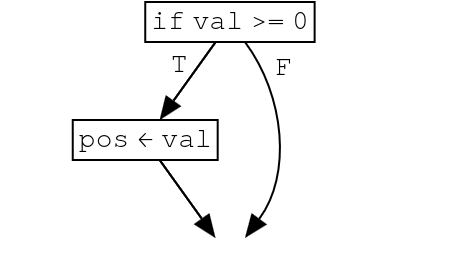
\includegraphics[scale=0.5]{./chapters/cfg.png}
  \centering
\end{figure}

Uma fase posterior da geração de código é a \emph{seleção de
instruções}, na qual a representação intermediária é traduzida em
instruções assembly. As instruções podem ser geradas como código
abstrato, no qual as variáveis são utilizadas como se fossem
registradores de hardware. Para o nosso exemplo, o resultado da
tradução para código de abstrato (x86-64) poderia ser o seguinte:

\begin{verbatim}
     cmp val, 0
     jl L1
     mov pos, val
L1:
\end{verbatim}

\section{Otimização de código}

A otimização de código é uma etapa cujo objetivo é melhorar a eficiência
de programas. Normalmente, ``melhor'' significa ``mais rápido'', embora
outros objetivos também sejam buscados, como reduzir o uso de memória
ou o consumo de energia do programa. A otimização pode ser aplicada
em praticamente todas as fases do compilador.

A otimização mais importante é a alocação de registradores, que
atribui variáveis à registradores de
hardware. Aplicar a alocação de registradores ao código assembly
acima poderia gerar o seguinte código assembly x86-64:

\begin{verbatim}
     cmp rax, 0
     jl L1
     mov rcx, rax
L1:
\end{verbatim}

Outra otimização que pode ser feita é usar uma sequência de
instruções, mais eficiente, que evite desvios.

\begin{verbatim}
cmp rax,0
cmovge rcx, rax
\end{verbatim}

\section{Visão geral de um compilador}

O compilador geralmente executa apenas uma parte da tarefa de
produzir código executável. Após gerar o código assembly para cada
uma das unidades de compilação (arquivos-fonte), um assembler é
utilizado para produzir módulos de código objeto que possuem
dependências entre si. Um linker resolve as dependências entre os
arquivos objeto e determina como modificar ou estender o código
assembly para que essas dependências sejam satisfeitas. Um loader,
frequentemente integrado ao sistema operacional, carrega então a
saída do linker na memória e produz uma imagem executável que o
processador pode interpretar.

\begin{figure}[H]
  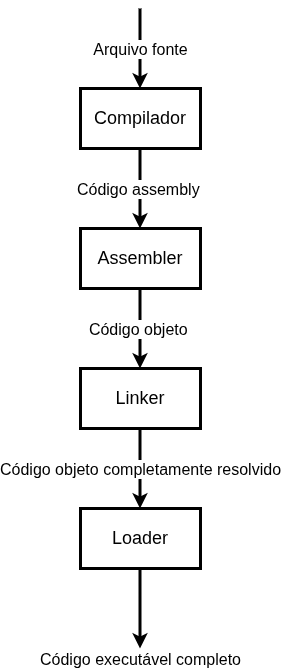
\includegraphics[scale=0.3]{./chapters/pipeline.png}
  \centering
\end{figure}

\section{Conclusão}

Neste capítulo, apresentamos uma visão geral do que é um compilador e
do desafio fundamental que ele enfrenta: traduzir programas de uma
linguagem de origem, projetada para seres humanos, para uma linguagem
de destino, otimizada para execução eficiente por hardware. Vimos
que, embora os compiladores sejam sistemas complexos, é possível
dominar essa complexidade dividindo o problema em fases menores e
mais gerenciáveis: análise léxica, sintática, semântica, geração
de código e otimização. Cada uma transformando gradualmente o
programa de sua representação original até o código de máquina final.
Ao longo deste material, exploraremos cada uma dessas fases em
detalhe, sempre buscando descrevê-las com precisão para que possamos
não apenas compreender seu funcionamento, mas também implementá-las
corretamente.
